	\documentclass[10pt,oneside]{CBFT_book}
	% Algunos paquetes
	\usepackage{amssymb}
	\usepackage{amsmath}
	\usepackage{graphicx}
	\usepackage{libertine}
	\usepackage[bold-style=TeX]{unicode-math}
	\usepackage{lipsum}

	\usepackage{natbib}
	\setcitestyle{square}

	\usepackage{polyglossia}
	\setdefaultlanguage{spanish}
	

	\everymath{\displaystyle}

	\usepackage{CBFT.estilo} % Cargo la hoja de estilo

	% Tipografías
	% \setromanfont[Mapping=tex-text]{Linux Libertine O}
	% \setsansfont[Mapping=tex-text]{DejaVu Sans}
	% \setmonofont[Mapping=tex-text]{DejaVu Sans Mono}

	%===================================================================
	%	DOCUMENTO PROPIAMENTE DICHO
	%===================================================================

\begin{document}

% =================================================================================================
\chapter{Introducción al momento angular (rotaciones)}
% =================================================================================================

El operador $\hat{L}$ será el encargado de realizar las rotaciones. Por el álgebra visto en la mecánica 
clásica sabemos que, dado un vector \vb{v} y una matriz ortogonal $R$ se tiene
\[
	\vb{v}' = R \vb{v} \qquad \text{con} \quad |\vb{v}'|=|\vb{v}|
\]
y 
\[
	|\vb{v}|^2 = V^t V = (V^t R^t) (R V) \qquad \text{pues} \quad R^tR=RR^t = \mathbb{1}
\]
puesto que es una matriz ortogonal. Luego se cumplen 
\[
	\text{clausura}	 \qquad (R_1R_2)(R_1R_2)^t = R_1R_2R_2^tR_1^t = \mathbb{1}
\]
el producto de dos matrices ortogonales es otra matriz ortogonal (aquella que cumple $R^rR=\mathbb{1}$)
\[
	\text{asociatividad} \qquad R_1(R_2R_3) = (R_1R_2)R_3
\]
\[
	\exists \; \text{identidad} \qquad R\mathbb{1} = \mathbb{1}R = R
\]
\[
	\exists \; \text{inversa} \qquad RR^{-1} = R^{-1}R = \mathbb{1} \qquad \text{con}\; R^{-1}\equiv R^t
\]
Esto define un grupo de matrices ortogonales que realiza rotaciones y se denomina $SO(3)$.

\subsection{No conmutatividad de las rotaciones clásicas}

Las rotaciones finitas no conmutan. Luego, el grupo de las rotaciones será un grupo abeliano
\[
	R_z(\varphi) = \begin{pmatrix}
	\cos(\varphi) & -\sin(\varphi) & 0 \\
	\sin(\varphi) & \cos(\varphi) & 0 \\
	0 & 0 & 1
	\end{pmatrix}
\]
\[
	R_x(\varphi) = \begin{pmatrix}
	1 & 0 & 0 \\
	0 & \cos(\varphi) & -\sin(\varphi) \\
	0 & \sin(\varphi) & \cos(\varphi)
	\end{pmatrix}
\]
\[
	R_y(\varphi) = \begin{pmatrix}
	\cos(\varphi) & 0 & \sin(\varphi) \\
	0 & 1 & 0 \\
	-\sin(\varphi) & 0 & \cos(\varphi)
	\end{pmatrix}
\]

\begin{figure}[!htb]
	\begin{center}
	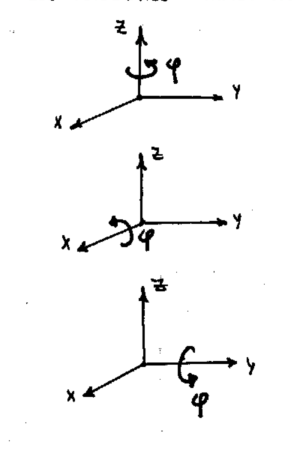
\includegraphics[width=0.5\textwidth]{images/teo2_10.pdf}
	\end{center}
	\caption{}
\end{figure} 

Si reemplazamos $\cos(\epsilon) \approx 1 - \epsilon^2/2$ y $\sin(\epsilon) \approx \epsilon$ hasta orden dos.
Se puede ver que las rotaciones, en torno a ejes diferentes, sólo conmutan a orden uno $(\epsilon)$ de manera 
que una rotación infinitesimal $d\varphi$ conmuta pero una rotación finita $\varphi$ no lo hace.

% =================================================================================================
\section{Rotaciones cuánticas}
% =================================================================================================

Para las rotaciones cuánticas se pedirá
\[
	D(\hat{n},d\phi) = \mathbb{1} - i \frac{\vb{J}\cdot\hat{n}}{\hbar}d\phi,
\]
rotación infinitesimal o bien
\[
	D(\hat{n},\theta) = \euler^{-i \vb{J}\cdot\hat{n}/\hbar \theta},
\]
para rotación finita. Donde $\hat{D}$ es el operador de las rotaciones y $\hat{J}$ es un momento angular 
general. Se postula de esta forma para que $\hat{D}$ cumpla las mismas propiedades que $R$ y la relación de 
conmutación
\[
	R_x R_y - R_y R_x = R_z (\epsilon^2) - \mathbb{1}
\]
\[
	D(\hat{x},\epsilon) D(\hat{y},\epsilon) - D(\hat{y},\epsilon) D(\hat{x},\epsilon) =
	D(\hat{z},\epsilon^2) - D(\mathbb{1})
\]
de modo que la cuenta lleva a  
\[
	J_x J_y - J_y J_x = i \hbar J_z
\]
la cual generalizando se llega a 
\[
	[J_i,J_j] = i \hbar \epsilon_{ijk} J_k
\]
que son las relaciones de conmutación generales para momento angular $\hat{J}$.

Para sistemas de spín $1/2$ es 
\[
	D(\hat{n},\phi) \equiv \euler^{-i/\hbar \vb{S}\cdot\hat{n} }
\]
Se puede ver que ante rotaciones cuánticas $D(\hat{n},\phi)$ los valores de expectación transforman como 
vectores
\[
	\begin{pmatrix} \Braket{S_x'} \\ \Braket{S_y'} \\ \Braket{S_z'}	\end{pmatrix} =	\begin{pmatrix} 
	\\
	 R(\hat{x},\phi) \\
	 \\
	\end{pmatrix}\begin{pmatrix} \Braket{S_x} \\ \Braket{S_y} \\ \Braket{S_z} \end{pmatrix}
\]

En general $\vb{J} = (J_x, J_y, J_z)$ se transforma como vector y entonces $\hat{J}$ es un operador vectorial.
Para spín $1/2$ es
\[
	\Ket{\alpha} = \Braket{+|\alpha}\Ket{+} + \Braket{-|\alpha}\Ket{-}
\]
\[
	D(\hat{z},\phi)\Ket{\alpha} = \euler^{-iS_z\phi/\hbar}\Braket{+|\alpha}\Ket{+} +
		\euler^{-iS_z\phi/\hbar} \Braket{-|\alpha}\Ket{-}
\]
\[
	D(\hat{z},\phi)\Ket{\alpha} = \Braket{+|\alpha} \euler^{-i\phi/2} \Ket{+} +
		\euler^{i\phi/2} \Braket{-|\alpha}\Ket{-}
\]
Si $\phi=2\pi$ (cosa que debiera dejar al ket incólume) se tiene 
\[
	D(\hat{z},2\pi) \Ket{\alpha} = - \Braket{+|\alpha}\Ket{+} - \Braket{-|\alpha}\Ket{-} = -\Ket{\alpha}
\]

Luego, esto es una muestra del carácter no-clásico del spin; una vuelta completa le cambia el signo al ket 
pero notemos cuidadosamente que el valor de expectación -- que es algo físico -- no varía. Esto muestra que 
el ket no puede tener sentido físico.

\subsection{Angulos de Euler}

Se define una serie de rotaciones 
\[
	1.\; R_{z}(\alpha) \qquad 2.\; R_{y'}(\beta)\qquad 3.\; R_{z'}(\gamma)
\]
lo cual equivale a
\[
	R(\alpha,\beta,\gamma) = R_{z'}(\gamma) R_{y'}(\beta) R_{z}(\alpha)
\]
\[
	\euler^{-i J_{z'}\gamma/\hbar} \euler^{-i J_{y'}\beta/\hbar}  \euler^{-i J_z\alpha/\hbar} 
	\Ket{\psi}
\]
\begin{figure}[!htb]
	\begin{center}
	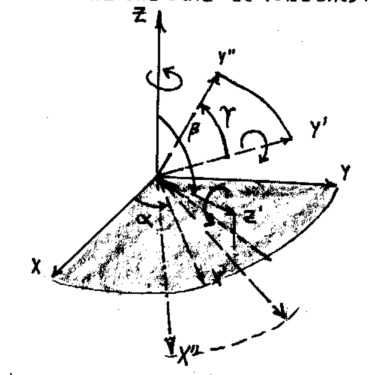
\includegraphics[width=0.5\textwidth]{images/teo2_11.pdf}
	\end{center}
	\caption{Los ángulos de Euler son una caracterización de una rotación general en 3D.}
\end{figure} 
Pero desconozco cómo operar en los ejes móviles $z',y'$
\[
	R_{y'}(\beta) = R_{z}(\alpha) R_{y}(\beta) R_{z}^{-1}(\alpha) 
\]
\[
	R_{z'}(\gamma) = R_{y'}(\beta) R_{z}(\gamma) R_{y'}^{-1}(\beta) 
\]
\[
	R(\alpha,\beta,\gamma) =
	R_{y'}(\beta) R_{z}(\gamma) \underbrace{R_{y'}^{-1}(\beta)R_{y'}(\beta)}_{\mathbb{1}}R_{z}(\alpha) 
\]
\[
	R(\alpha,\beta,\gamma) =
	R_{z}(\alpha) R_{y}(\beta) R_{z}^{-1}(\alpha) R_{z}(\gamma) R_{z}(\alpha)  
\]
\[
	R(\alpha,\beta,\gamma) = R_{z}(\alpha) R_{y}(\beta) R_{z}(\gamma)
\]
Rotación equivalente a [1] pero para ejes fijos, puesto que en mecánica cuántica sabemos rotar en torno a 
ejes fijos.

Los ángulos de Euler son la caracterización de una rotación general en 3D.

Entonces nuestra rotación en 3D cuántica será:
\[
	D(\alpha,\beta,\gamma) = D_z(\alpha) D_y(\beta) D_z(\gamma)  =
	\euler^{-i J_z\alpha/\hbar} \euler^{-i J_y\beta/\hbar} \euler^{-i J_z\gamma/\hbar}
\]

\subsection{Autoestados y autovalores de J}

Partimos de 
\[
	[J_i, J_j] =  i\hbar \epsilon_{ijR}J_R
\]
y
\[
	J^2 = J^2_x + J^2_y + J^2_z, \qquad  [J^2,J] = 0
\]
siendo la última muy importante y probándose por evaluación directa. Lleva a 
\[
	[J^2,J_i^n] = 0 \qquad \text{con} \; i=x,y,z \;\; n\in\mathbb{N}
\]

Se eligen $J^2, J_z$ como observables que conmutan 
\[
	J^2 \Ket{a,b} = a\Ket{a,b} \qquad \qquad J_z \Ket{a,b} = b\Ket{a,b}
\]
siendo $a$ autovalor de $J^2$ y $b$ de $J_z$.

Definiremos los operadores de subida y de bajada
\[
	J_{\pm} \equiv J_x \pm J_y
\]
que verifican 
\[
	[ J_+, J_- ] = 2\hbar J_z \qquad [ J_z, J_\pm]= \pm \hbar J_{\pm} \qquad [J_{\pm}, J^2 ] = 0
\]
Entonces se tiene 
\[
	J^2( J_\pm \Ket{a,b}) = J_\pm J^2 \Ket{a,b} = a J_\pm \Ket{a,b} \longrightarrow 
		J_\pm \Ket{a,b} = \Box \Ket{a,b}
\]
\[
	(J_zJ_\pm - J_\pm J_z) \Ket{a,b} = \pm\hbar J_\pm \Ket{a,b}
\]
\[
	J_z (J_\pm \Ket{a,b}) = (b\pm\hbar)(J_\pm \Ket{a,b}) \longrightarrow 
		J_\pm \Ket{a,b} = \boxdot \Ket{a,b\pm\hbar}
\]
\[
	J_{\pm} \Ket{a,b} = c_{\pm} \Ket{a,b\pm\hbar}
\]
\[
	J_+\Ket{a,b} = c_+\Ket{a,b+\hbar} \;\qquad\; J_-\Ket{a,b} =  c_- \Ket{a,b-\hbar}
\]
sube el $J_z$ en una unidad de $\hbar$ o bien baja el $J_z$ en una unidad de $\hbar$.
\[
	J_+J_- = J_x^2 + iJ_yJ_x - iJ_xJ_y + J_y^2 , \qquad J_-J_+ = J_x^2 - iJ_yJ_x + iJ_xJ_y + J_y^2
\]
\[
	J^2 = J_z^2 + \frac{1}{2}(J_+J_- + J_-J_+ ) , \qquad 
		J^2 - J_z^2 = \frac{1}{2}(J_+J_+^\dagger + J_+^\dagger J_+ )
\]
\[
	\Braket{a,b|J^2 - J^2_z|a,b} =  1/2 \Braket{a,b|J_+J_+^\dagger + J_+^\dagger J_+|a,b}
\]
\[
	(a-b^2)\Braket{a,b|a,b} = 1/2 \left[ \Braket{a,b|J_+J_+^\dagger|a,b} + 
		\Bra{a,b|J_+^\dagger} J_+\Ket{a,b} \right] 
\]
\[
	(a-b^2)\Braket{a,b|a,b} = |J_+^\dagger\Ket{a,b}|^2 \geq 0, \qquad \Rightarrow a \geq b^2
\]
hay cota para $b$.
\[
	J_+ \Ket{a,b_M} = 0
\]
Como no puede seguir subiendo debe dar el ket nulo 
\[
	J_-J_+ \Ket{a,b_M} = 0
\]
pero
\[
	J_-J_+ = J^2_x + J^2_y + i[J_x, J_y]  = J^2 - J^2_z - \hbar J_z
\]
\[
	( J^2 - J^2_z  -\hbar J_z) \Ket{a,b_M}  = 0	
\]
\[
	( a - b_M^2 - \hbar b_M ) \Ket{a,b_M}  = 0	
\]
\[
	a = b_M ( b_M -\hbar )
\]
\[
	J_- \Ket{a,b_m} = 0
\]
y como no puede seguir bajando debe dar el ket nulo
\[
	J_+J_- \Ket{a,b_m} = 0
\]
\[
	J_+J_- =  J^2 - J^2_z + \hbar J_z
\]
\[
	( J^2 - J^2_z + \hbar J_z) \Ket{a,b_m} = ( a - b_m^2 + \hbar b_m) \Ket{a,b_m} = 0
\]
\[
	b_M( b_M + \hbar ) = b_m( b_m -\hbar )
\]
tiene solución $b_M-b_m = -\hbar$ si $b_M + b_m \neq 0$ 
pero esto es absurdo de manera que $b_M = b_m$.
Entonces
\[
	-b_m = b_M  \qquad \Rightarrow \qquad -b_M \leq b \leq b_M
\]

Luego,
\[
	\Ket{a,b_m} \longrightarrow \Ket{a,b_M}
\]
y como $J_+$ sube de a un $\hbar$ será
\[
	b_M = b_m + n\hbar
\]
y entonces
\[
	b_M = \frac{n\hbar}{2} = \frac{n}{2} \hbar = j \hbar
\]
y se da que $j$ es entero o semientero.

Definiremos 
\[
	b_M \equiv j \hbar \qquad a \equiv j (j+1) \hbar^2 \qquad -j\hbar \leq b \leq j\hbar
\]
pero como $b/\hbar = m$
\[
	b_M \equiv j \hbar \qquad a \equiv j (j+1) \hbar^2 \qquad -j \leq m \leq j
\]
\[
	m = (-j,-j+1,-j+2,...,j-1,j) \qquad 2j+1 \text{valores de} \; m
\]
\[
	J^2 \Ket{j,m} = j( j+1 )\hbar^2\Ket{j,m} \qquad J_z \Ket{j,m} = m \hbar \Ket{j,m}
\]

\subsection{La normalización de $J_\pm$}

\[
	J_+\Ket{j,m} = c_+ \Ket{j,m+1} \qquad \qquad J_-^\dagger = J_+
\]
\[
	\Braket{j,m|J_-J_+|j,m} = \Braket{j,m|J_+^\dagger J_+|j,m} = |c_+|^2
\]
\[
	\Braket{j,m|J^2 - J_z^2 - \hbar J_z|j,m} = j(j+1)\hbar^2 - m^2\hbar^2 -\hbar^2 m = |c_+|^2
\]
\[
	c_+ = \hbar\sqrt{j(j+1)-m(m+1)} = \hbar \sqrt{(j-m)(j+m+1)}
\]
\[
	\Braket{j,m|J_+J_-|j,m} = \Braket{j,m|J_-^\dagger J_-|j,m} = |c_-|^2
\]
\[
	= j(j+1)\hbar^2 - m^2\hbar^2 + m\hbar^2 = |c_-|^2
\]
\[
	c_- = \hbar\sqrt{j(j+1)-m(m-1)} = \hbar \sqrt{(j+m)(j-m+1)}
\]
\[
	J_+ \Ket{j,m} = \hbar \sqrt{(j-m)(j+m+1)}\Ket{j,m+1} \qquad 
	J_- \Ket{j,m} = \hbar \sqrt{(j+m)(j-m+1)}\Ket{j,m-1}
\]

\subsection{Elementos de matriz de $J^2, J_z, J_+$}

Asumiendo normalización de $\Ket{j,m}$ se tiene 
\[
	\Braket{j',m'|J^2|j,m} = j(j+1)\hbar^2 \delta_{jj'} \delta_{m' m}
\]
\[
	\Braket{j',m'|J_z|j,m} = m \hbar \delta_{jj'} \delta_{m' m}
\]

\subsection{Elementos de matriz de $\mathcal{D}(R)$}

Ahora queremos ver cual es la forma de los elementos de matriz de $\mathcal{D}(R)$
\[
	\mathcal{D}(R) = \euler^{i \vb{J}\cdot\vec{n}\phi/\hbar}
\]
siendo que $\mathcal{D}(R)$ tiene por efecto rotar el sistema físico.
Lo primero que hay que notar es que 
\[
	\Braket{j',m'|\mathcal{D}(R)|j,m}  \propto \delta_{jj'}
\]
porque $[J^2,J_i]=0$ y entonces $[J^2,J_i^n]=0$ y 
\[
	\mathcal{D}(R) = f(J_i) \; \longrightarrow \; [ J^2, \mathcal{D}(R) ] = 0
\]
y 
\[
	\mathcal{D}^{(j)}_{m' m} =  \Braket{j,m'|\euler^{i \vb{J}\cdot\vec{n}\phi/\hbar}|j,m} 
\]
es una matriz para cada $j$ fijo con $\{ (2j+1)\times(2j+1)=\text{dimensión}\}$
\[
	\mathcal{D}(R)\Ket{j,m} = \sum_{m'} \ket{j,m'}\Braket{j,m'|\euler^{i \vb{J}\cdot\vec{n}\phi/\hbar}|j,m} 
	= \sum_{m'} \mathcal{D}^{(j)}_{m' m}(R) \Ket{j,m'} 
\]
pero las rotaciones no cambian el $j$, $\mathcal{D}(R)$ conecta estados con la misma $j$ y $\mathcal{D}(R) 
\in (2j+1)\times(2j+1)$ 
\[
	\mathcal{D}(R)\Ket{j,m} = \sum_{m'} \mathcal{D}^{(j)}_{m' m}(R) \Ket{j,m'} 
\]

La matriz de $\mathcal{D}(R)$ (no caracterizada por un único $j$) puede ponerse en forma diagonal por bloques:
\[
\begin{matrix} \qquad j' \quad j'' \quad j''' \end{matrix}
\]
\[
	\mathcal{D}(R) = \begin{pmatrix}
	\; \Box & 0 & 0 & \\
	\; 0 & \Box & 0 & \\
	\; 0 & 0 & \Box & \\
	\; & & & \vdots
	\end{pmatrix} \begin{matrix} j' \\ j'' \\ j'''\\ \\ \end{matrix}
\]
con cada bloque de $(2j+1)\times(2j+1)$ , pero siendo cada bloque irreducible. Las matrices de rotación con 
$j$ fijo forman un grupo. $\mathcal{D}_{m'm}^{(j)}(R)$ son los elementillos de la matriz.
\[
	\Ket{j,m} \underbrace{\longrightarrow}_{\text{Rotación}} \mathcal{D}(R)\Ket{j,m} =
	 \sum_{m'} \mathcal{D}^{(j)}_{m' m}(R) \Ket{j,m'} 
\]
donde el $\mathcal{D}^{(j)}_{m' m}(R)$ es la amplitud de hallar al $\Ket{j,m}$ rotado en $\Ket{j,m'}$

\subsection{Forma explícita del operador $\mathcal{D}(R)$}

Los ángulos de Euler permitieron caracterizar la rotación más general. Entonces 
\[
	\mathcal{D}^{(j)}_{m' m} = 
	\Braket{j,m'|\euler^{-iJ_z\alpha/\hbar} \euler^{-iJ_y\beta/\hbar} \euler^{-iJ_z\gamma/\hbar} |j,m}
\]
\[
	\mathcal{D}^{(j)}_{m' m} = \euler^{-i(-m'\alpha + m\gamma)}
	\underbrace{\Braket{j,m'| \euler^{-iJ_y\beta/\hbar}  |j,m}}_{d_{m'm}^{(j)}}
\]
siendo el primer factor una fase.
En los $d_{m'm}^{(j)}$ está la dificultad de la cuenta.

% =================================================================================================
\section{Formalismo de spinores de Pauli}
% =================================================================================================

Apropiado para trabajar con sistemas de spín $1/2$. Estos sistemas son casos particulares de momento angular,
\[
	j = 1/2 \qquad m=-\frac{1}{2},+\frac{1}{2}
\]
y se definen los spinores $\chi_\pm$ como
\[
	\Ket{+} \equiv  \begin{pmatrix} 1 \\ 0  \end{pmatrix} \equiv  \chi_+ \qquad \qquad
	\Ket{-} \equiv  \begin{pmatrix} 0 \\ 1  \end{pmatrix} \equiv  \chi_-
\]
\[
	\Ket{\alpha} = \begin{pmatrix}   \Braket{+|\alpha} \\ \Braket{-|\alpha}  \end{pmatrix}
\]
\[
	\Bra{\alpha} = \begin{pmatrix}  \; \Braket{+|\alpha} \quad \Braket{-|\alpha} \;  \end{pmatrix}
\]

Para spín $1/2$ podemos tomar $\vb{J} = \vb{S}$ por la analogía de las relaciones de conmutación.
A su vez 
\[
	\vb{S} = \frac{\hbar}{2} \vec{\sigma} \qquad \text{con} \qquad \vec{\sigma} \equiv 
	\begin{pmatrix} \; \sigma_x, \sigma_y, \sigma_z \; \end{pmatrix}
\]
que es una especie de vector 
\[
	\vec{\sigma}  =
	\begin{bmatrix}
	 \begin{pmatrix} 0 & 1 \\ 1 & 0 \end{pmatrix}, \begin{pmatrix} 0 & -i \\ i & 0 \end{pmatrix},
	 \begin{pmatrix} 1 & 0 \\ 0 & -1 \end{pmatrix} 
	\end{bmatrix}
\]
Luego esta equivalencia provee expresión de los operadores $S_i$ en términos de matrices de $2\times 2$, así:
\[
	\frac{i}{2}[ J_- - J_+] = J_y = S_y = \frac{\hbar}{2} \sigma_y
\]
siendo que los $J_y$ y $S_y$ actúan sobre kets y el $\sigma$ sobre spinores.

Las matrices de Pauli cumplen las propiedades básicas siguientes 
\[
	\sigma^2_i = \mathbb{1} \qquad \sigma_i^\dagger = \sigma_i
\]
\[
	[ \sigma_, \sigma_j ] = i2\varepsilon_{ijR}\sigma_R \qquad \{\sigma_, \sigma_j \}= \delta_{ij}
\]
\[
	\sigma_i^n = \begin{cases} \mathbb{1} \quad n \; \text{par} \\ \sigma_i \quad n \; \text{impar} 
\end{cases}
\]
\[
	\Ket{+} \equiv \Ket{j=1/2 , m = 1/2} \qquad \Ket{-} \equiv \Ket{j=1/2 , m = -1/2} 
\]
\[
	(\vec{\sigma}\cdot\vb{a})(\vec{\sigma}\cdot\vb{b}) = 
		(\vb{a}\cdot\vb{b}) + i \vec{\sigma}\cdot(\vb{a}\times\vb{b})
\]

\subsection{Aplicación a las rotaciones}

\[
	\mathcal{D}(\hat{n},\phi) = \euler^{-i \vb{J}\cdot\hat{n}\phi/\hbar} = \euler^{-i\vec{\sigma}\cdot\hat{n}\phi/2}
\]
pero 
\[
	(\vec{\sigma}\cdot\hat{n})^n = \begin{cases}
	                                \vec{\sigma}\cdot\hat{n} \qquad n \; \text{impar} \\
	                                \mathbb{1} \qquad \quad \; n \; \text{par} 
	                               \end{cases}
\]
\[
	\euler^{-i\vec{\sigma}\cdot\hat{n}\phi/2} = 1 - i\vec{\sigma}\cdot\hat{n} \:\frac{\phi}{2} - 
	\frac{1}{2!} (\vec{\sigma}\cdot\hat{n})^2\left(\frac{\phi}{2}\right)^2 + 
	\frac{i}{3!} (\vec{\sigma}\cdot\hat{n})^3\left(\frac{\phi}{2}\right)^3 - ...
\]
\[
	\mathcal{D}(\hat{n},\phi) = \euler^{-i\vec{\sigma}\cdot\hat{n}\phi/2} =
	\mathbb{1}\cos\left(\frac{\phi}{2}\right) - i\vec{\sigma}\cdot\hat{n}\sin\left(\frac{\phi}{2}\right)
\]
es el operador de rotación para sistemas de spin $1/2$ (donde $\mathbb{1} \in 2\times 2$). Con esta expresión podemos 
evaluar 
$d^{j=1/2}_{m'm}(\beta)$
\[
	d^{1/2}(\beta) = \begin{pmatrix}
	     \cos(\beta/2) & -\sin(\beta/2)\\
	     \sin(\beta/2) & \cos(\beta/2)
	    \end{pmatrix}
\]
donde hemos usado los resultados 
\[
	\cos(x) = \sum_{n=0}^\infty \frac{(x)^{2n+1}}{(2n+1)!}(-1)^n \qquad 
		\sin(x) = \sum_{n=0}^\infty \frac{(x)^{2n}}{(2n)!}(-1)^n
\]

En el caso general el operador de rotación para sistemas de spin $1/2$ lucirá:
\[
	\begin{matrix} \qquad\qquad \Ket{+} \qquad\qquad\qquad\qquad \Ket{-} \end{matrix}
\]
\[
	\mathcal{D}^{j=1/2} (\alpha,\beta,\gamma) = \begin{pmatrix}
	        \euler^{-\frac{i}{2}(\alpha + \gamma)} \cos\left(\frac{\beta}{2}\right) & 
			- \euler^{-\frac{i}{2}(\alpha - \gamma)} \sin\left(\frac{\beta}{2}\right) \\
	        \euler^{-\frac{i}{2}(\gamma -\alpha )} \sin\left(\frac{\beta}{2}\right) & 
			\euler^{\frac{i}{2}(\alpha + \gamma)} \cos\left(\frac{\beta}{2}\right)
	       \end{pmatrix} 
	       \begin{matrix} \Ket{+} \\ \\  \Ket{-} \end{matrix}
\]

\subsection{Ejemplo}

\[
	d^{1/2}(\pi/2) = \begin{pmatrix}
	                  \sqrt{2}/2 & -\sqrt{2}/2 \\
	                  \sqrt{2}/2 & \sqrt{2}/2
	                 \end{pmatrix}
\]
de manera que 
\[
	d^{1/2}(\pi/2)\chi_{+} = \frac{\sqrt{2}}{2}\begin{pmatrix} 1 & -1 \\  1 & 1 \end{pmatrix}
	                                           \begin{pmatrix}  1 \\ 0  \end{pmatrix} 
				= \frac{\sqrt{2}}{2} \begin{pmatrix}  1 \\ 1 \end{pmatrix} 
\]
\[
	d^{1/2}(\pi/2)\chi_{+} = \frac{\sqrt{2}}{2} (\chi_+ + \chi_- )  = \frac{1}{2} \left( \Ket{+} + \Ket{-} \right)
\]
\[
	d^{1/2}(\pi/2)\chi_{+} = \Ket{S_x ; + }
\]
Este resultado es intuitivamente lógico.


\subsection{Rotaciones en sistemas con $j=1$}

Ahora tenemos 
\[
	j=1 \qquad m = -1,0,1
\]
recordando $J_y$ en términos de escaleras
\[
	J_y = \frac{J_+ - J_i}{2i}
\]
de modo que 
\[
	\begin{matrix} \quad \Ket{1\;1} \quad \Ket{1\;0} \quad \Ket{1\;-\kern-1mm 1} \end{matrix}
\]
\[
	J_y = \frac{i\hbar}{\sqrt{2}} \begin{pmatrix}
	                               \quad 0 & \quad -1 \quad & 0 \quad \\
	                               \quad 1 & \quad 0 \quad & -1 \quad \\
	                               \quad 0 & \quad 1 \quad & 0 \quad
	                              \end{pmatrix} 
	     \begin{matrix}  \Ket{1\;1} \\ \Ket{1\;0} \\ \Ket{1\;-\kern-1mm 1} \end{matrix}
\]
\[
	\euler^{-i\frac{J_y}{\hbar}\beta} = 1 + -\frac{J_y}{\hbar}\beta + 
		(-i)^2\left(\frac{J_y}{\hbar}\beta\right)^2\frac{1}{2!} + 
		(-i)^3\left(\frac{J_y}{\hbar}\beta\right)^3\frac{1}{3!} + ...
\]
\[
	\euler^{-i\frac{J_y}{\hbar}\beta} = 1 - \frac{J_y}{\hbar}\beta -
		\frac{1}{2!} \left(\frac{J_y}{\hbar}\beta\right)^2 -
		\frac{i}{3!}\left(\frac{J_y}{\hbar}\beta\right)^3 + ...
\]
\[
	\left( \frac{J_y}{\hbar} \right)^n = \begin{cases}
	                                      \left( \frac{J_y}{\hbar} \right) \quad n \; \text{impar} \\
	                                      \left( \frac{J_y}{\hbar} \right)^2 \quad n \; \text{par}
	                                     \end{cases}
\]
\[
	\euler^{-i\frac{J_y}{\hbar}\beta} = 1 -  \left( \frac{J_y}{\hbar} \right)^2 (1-\cos(\beta)) -
	i \left( \frac{J_y}{\hbar} \right) \sin(\beta)  = d^{j=1}(\beta)
\]
acá lo vemos como operador (es notación), $d_{m'm}^{j=1}(\beta)$ simboliza la matriz
\[
	\begin{matrix} \Ket{1\;1} \qquad\qquad\quad \Ket{1\;0} \qquad\qquad \Ket{1\;-\kern-1mm 1} \end{matrix}
\]
\[
	d^{j=1}(\beta) =
	\begin{pmatrix}
	\displaystyle \frac{1}{2}( 1 + \cos(\beta)) & -\frac{1}{\sqrt{2}}\sin(\beta) & \frac{1}{2}( 1 - 
\cos(\beta) ) \\
	\displaystyle{\frac{1}{\sqrt{2}}\sin(\beta)} & \cos(\beta) & -\frac{1}{\sqrt{2}}\sin(\beta) \\
	\displaystyle{\frac{1}{2}(1 - \cos(\beta))} & \frac{1}{\sqrt{2}}\sin(\beta) & \frac{1}{2}  ( 1 + 
\cos(\beta) )
	\end{pmatrix} \begin{matrix} \Ket{1\;1} \\ \\ \Ket{1\;0} \\ \\ \Ket{1\;-\kern-1mm 1} \end{matrix}
\]

% =================================================================================================
\section{Momento angular orbital}
% =================================================================================================

\[
	\vb{L} = \vb{x} \times \vb{p}
\]
verifica el álgebra de $\vb{J}$,
\[
	[ L_i, L_j ] = i\hbar \epsilon_{ijR} L_R \qquad L_i = \epsilon_{ijk}x_jp_k
\]
\[
	L_z = xp_y - yp_x
\]
Consideremos ahora una rotación en torno a $z$, en un $\delta\phi$,
\[
	\left( 1 - \frac{iL_z\delta\phi}{\hbar} \right) \Ket{x',y',z'} =
	1 - \frac{iP_y}{\hbar}(x\delta\phi) + \frac{iP_x}{\hbar}(y\delta\phi) \Ket{x',y',z'}
\]
\[
	= \left[ 1 - \frac{i}{\hbar}\left( P_y x\delta\phi - P_x y\delta\phi \right)\right] \Ket{x',y',z'}
\]
esto es una traslación en $\hat{x},\hat{y}$,
\[
	(1-i\frac{L_z}{\hbar}\delta\phi) \Ket{x',y',z'} = \Ket{x'-y'\delta\phi,y'+x'\delta\phi,z'}
\]

Esta traslación es debida a una rotación infinitesimal en $\delta\phi$ torno a $z$ entonces genera las 
rotaciones clásicas en torno a $z$.
\[
	\Psi_\alpha(\vb{x}') = \Braket{x',y',z'|\alpha} \underbrace{\longrightarrow}_{\text{Rotamos en z}}
	\Braket{x',y',z'|1-\frac{iL_z\delta\phi}{\hbar}|\alpha} = \Braket{x'+y'\delta\phi,y'-x'\delta\phi,z'|\alpha}
\]
y en coordenadas esféricas,
\[
	\Psi_\alpha(\vb{x}') = \Braket{r,\theta,\phi|\alpha} 
	\underbrace{\longrightarrow}_{\text{Rotamos en z}} \Braket{r,\theta,\phi-\delta\phi|\alpha}
\]

Podemos hallar una expresión para $L_z$ en esféricas:
\[
	\Braket{r,\theta,\varphi|1-\frac{L_z\delta\phi}{\hbar}|\alpha} \approx
	\Braket{\phi|\alpha} -\dpar{}{\phi}\Braket{\phi|\alpha}\delta\phi
\]
identificamos 
\[
	\Braket{\vb{r}|-\frac{iL_z}{\hbar}|\alpha} = -\dpar{}{\phi}\Braket{\vb{r}|\alpha}
\]
\[
	L_z =  -i\hbar\dpar{}{\phi}
\]
operador $L_z$ en esféricas.

Esta construcción usa que 
\[
	\dpar{}{\phi} \Braket{\phi|\alpha} \approx 
	\frac{\Braket{\phi+\delta\phi|\alpha}-\Braket{\phi|\alpha}}{\delta\phi} =
	\frac{\Braket{\phi|\alpha} -\Braket{\phi-\delta\phi|\alpha}}{\delta\phi}
\]
y luego se despeja de la última $\Braket{\phi-\delta\phi|\alpha}$.

Usando 
\[
	L^2 = L_z^2 + \frac{1}{2}\left( L_+L_- + L_-L_+ \right)
\]
se llega a 
\[
	\Braket{r,\theta,\phi|L^2|\alpha} = -\hbar^2\left[ \frac{1}{\sin^2 \theta}\dpar[2]{}{\phi} +
	\frac{1}{\sin \theta} \dpar{}{\theta}[\sin\theta\dpar{}{\theta} ]\right]
	\Braket{r,\theta,\varphi|\alpha}
\]
\[
	L^2 = -\hbar^2 r^2 \nabla^2_{\theta,\varphi}
\]
donde $\nabla^2_{\theta,\varphi}$ es la parte angular del laplaciano en coordenadas esféricas.
Esto puede obtenerse también partiendo de 
\[
	L^2 = \vb{x}^2\vb{p}^2 - (\vb{x}\cdot\vb{p})^2 + i\hbar \vb{x}\cdot\vb{p}
\]

Sea un $H$ de partícula, sin spín, sujeta a potencial simétricamente esférico. Sabemos que la función de onda 
$\Psi_\alpha(\vb{r}')$ es separable en coordenadas esféricas, entonces:
\[
	\Braket{\vb{r}|n,l,m} = R_{nl}(r)Y_l^m(\theta,\phi)
\]
\[
	\Braket{\vb{r}|n,l,m} = (\Bra{{r}}\otimes\Bra{\theta,\phi})(\Ket{n,l,m})=
	\Braket{r|n,l,m}\Braket{\theta,\phi|l,m}
\]

Cuando el H es esféricamente simétrico (como en un potencial central) se tiene 
\[
	[H,L_z] = [H,L^2] = 0
\]

Trabajaremos solamente en la parte angular  $\Ket{\theta,\varphi} \equiv \Ket{\hat{n}}$
\[
	\Braket{\hat{n}|\ell,m} = Y_l^m(\theta,\phi) = Y_l^m(\hat{n})
\]
que es la amplitud de hallar $\Ket{\ell,m}$ en la dirección $\hat{n}$.

Podemos vincular ahora los armónicos esféricos con los autoestados de $L_z,L^2$
\[
	L_z \Ket{\ell,m} = m\hbar\Ket{\ell,m}
\]
de manera que 
\[
	\Braket{\hat{n}|L_z|\ell,m} = m\hbar \Braket{\hat{n}|\ell,m} =
	-i\hbar \dpar{}{\phi} \Braket{\hat{n}|\ell,m}
\]
y entonces 
\[
	Y_l^m(\theta,\phi) \propto \euler^{im\phi}.
\]
\[
	L^2 \Ket{\ell,m} = l(l+1)\hbar^2\Ket{\ell,m}
\]
y de modo ídem
\[
	\Braket{\hat{n}|L^2|\ell,m} = l(l+1)\hbar^2\Braket{\hat{n}|\ell,m}
\]
\[
	( -\hbar^2 r^2 \nabla^2_{\theta,\phi} + l(l+1)\hbar )\Braket{\hat{n}|\ell,m} = 0 
\]
Entonces, con la ortogonalidad
\[
	\longrightarrow \Braket{l',m'|l,m} = \delta_{l'l} \delta_{m'm}
\]
y con la completitud 
\[
	\longrightarrow \int d\Omega \Ket{\hat{n}}\Bra{\hat{n}} = 1
\]
de manera que llegamos a 
\[
	\int d\Omega \Braket{l',m'|\hat{n}} \Braket{\hat{n}|l,m} = \delta_{l'l} \delta_{m'm}   \qquad 
	\int d\Omega Y_l^{m*}(\theta,\phi)  Y_l^m(\theta,\phi)  = \delta_{l'l} \delta_{m'm}
\]

Podemos hallar una expresión para 
\[
	\Braket{\hat{n}|L_+|l,l} = 0
\]
\[
	-i\hbar\euler^{i\phi}(i\dpar{}{\theta}-\cot\theta\dpar{}{\phi})\Braket{\hat{n}|l,l} = 0 \Rightarrow
	Y_l^m(\theta,\phi)  = c_l \euler^{il\phi}\sin^l\theta
\]

Luego usamos $L_-$ para hallar sucesivamente los demás $Y^m_\ell$
\[
	\frac{\Braket{\hat{n}|L_-|l,m} }{\sqrt{(l+m)(l-m+1)}} = \Braket{\hat{n}|l,m-1} 
\]
y por este camino se llega a 
\[
	Y_l^m(\theta,\phi) = \frac{(-1)^l}{2^ll!}\sqrt{\frac{(2l+1)(l+m)!}{4\pi(l-m)!}} \euler^{im\phi} 
\frac{1}{\sin\theta}
	\dtot{^{l-m}}{(\cos^{l-m}\theta)}(\sin\theta)^{2l}
\]
con 
\[
	Y_l^{-m}(\theta,\phi) = (-1)( Y_l^m(\theta,\phi) )^* \qquad 
	Y_l^0(\theta,\phi) = \sqrt{\frac{2l+1}{4\pi}}P_l(\cos\theta)
\]

En el caso de momento angular orbital $\ell$ no puede ser semientero porque entonces $m$ sería semientero y 
en una vuelta de $2\pi$
\[
	\euler^{im2\pi} = -1
\]
entonces $\psi$ no será univaluada

Además,
\[
	\Braket{\vb{x}|\euler^{-iL_z2\pi/\hbar}|\alpha} = \Braket{\vb{x}|\alpha} \qquad \text{(no hay signo menos)}
\]


% \bibliographystyle{CBFT-apa-good}	% (uses file "apa-good.bst")
% \bibliography{CBFT.Referencias} % La base de datos bibliográfica

\end{document}
